\subsection{One-shot change of variables}\label{sec:cov}

The naive stable search keeps $z$ and searches in rank $3$. A change of variables uses $z$ once, to remove $x$ or $y$,
and then searches in rank $2$ again.

\begin{definition}[Change of variables]\label{def:cov}
Let $P=\pres{x,y}{r_1,r_2}$ and let $w$ be a word in $x,y$ of length at least $2$.
\begin{enumerate}
  \item \emph{Stabilize}: $P_w=\pres{x,y,z}{r_1,\ r_2,\ z^{-1}w}$ (Definition~\ref{def:stab}).
  \item \emph{Substitute}: replace non-overlapping occurrences of $w^{\pm1}$ in $r_1,r_2$ by $z^{\pm1}$ and freely
  reduce. Call the results $r_1',r_2'$.
  \item \emph{Eliminate}: choose one of $r_1',r_2',z^{-1}w$ in which a generator $g\in\{x,y\}$ occurs exactly once.
  Write it cyclically as $g^{\epsilon}s$, with $g$ not in $s$, so that $g=s^{-\epsilon}$ in the group. Substitute
  $s^{-\epsilon}$ for $g$ in the other two relators and delete the chosen one.
\end{enumerate}
The result is a presentation $P'$ on the two generators $\{x,y,z\}\setminus\{g\}$, the \emph{image} of $P$. We rename
them $x,y$ and search $P'$ with LENGTH.
\end{definition}

\begin{example}
Let $P=\pres{x,y}{y^{-5}x^{-1}y^{4}x,\ y^{-2}xy^{-1}xy^{-1}x^{-1}}$ and $w=x^{-1}y$. Substituting $z$ for
$w$ ($3$ occurrences) gives
\[
P_w\ \to\ \pres{x,y,z}{y^{-5}zy^{3}x,\ \ y^{-1}z^{-2}y^{-1}x^{-1},\ \ z^{-1}x^{-1}y}.
\]
In the first relator $x$ occurs once: $x=y^{-3}z^{-1}y^{5}$. Substituting it into the other two and renaming
$y,z$ as $x,y$ gives the image
\[
P'=\pres{x,y}{x^{-1}y^{-2}x^{-6}yx^{3},\ \ y^{-1}x^{-5}yx^{4}}.
\]
\end{example}

\begin{definition}[One-shot CoV]\label{def:oneshot}
The words $w$ are the cyclic subwords of $r_1$ and $r_2$ of length at least $2$, one of each pair $\{w,w^{-1}\}$,
except those whose substitution leaves a relator with fewer than $3$ letters. Step 2 substitutes every
non-overlapping occurrence, read left to right; step 3 tries $g=x$ and $g=y$ and every relator in which $g$ occurs once.
Each choice gives one image, and the images are ordered by $|w|$, then by $w$. The one-shot policy runs LENGTH with
$10^3$ units on $P$ itself, then on the images in this order, $10^3$ units each, and stops at the first solve or after
$10^4$ units in total. $P$ is searched at cap $24$, an image at cap $\max(24,\ \text{longest relator of }P'+16)$.
\end{definition}

On MS640 a presentation has $8$ to $174$ images (median $56$). The policy reaches at most the first $9$ of them, since
$P$ takes the first $10^3$ units.

\paragraph{Score.} Table~\ref{tab:cov_oneshot} compares the policy with LENGTH on $P$ at the same total budget of
$10^4$ units. Every solve was replayed: an AC path on $P$, a stable certificate by redoing the change of variables and
then the path on $P'$.

\begin{table}[ht]
\centering
\small
\begin{tabular}{lrrrrrr}
\toprule
& & \multicolumn{2}{c}{AC path of $P$} & & & LENGTH\\
\cmidrule(lr){3-4}
benchmark & solved & from $P$ & from $\varphi(P)$ & stable certificate & units spent & at $10^4$\\
\midrule
MS640 & $584$ & $554$ & $0$ & $30$ & $693{,}162$ & $606$\\
bench60 & $39$ & $29$ & $0$ & $10$ & $246{,}744$ & $40$\\
ladder100 & $46$ & $11$ & $13$ & $22$ & $734{,}766$ & $20$\\
\bottomrule
\end{tabular}
\caption{One-shot CoV, $10^3$ units per search and $10^4$ per presentation. Units spent: summed over the benchmark,
failures included.}
\label{tab:cov_oneshot}
\end{table}

\begin{table}[ht]
\centering
\small
\begin{tabular}{llrrrr}
\toprule
& & \multicolumn{2}{c}{units to solve} & \multicolumn{2}{c}{S-moves}\\
\cmidrule(lr){3-4}\cmidrule(lr){5-6}
benchmark & solved by & median & max & median & max\\
\midrule
MS640 & $P$ & $9$ & $990$ & $8$ & $101$\\
& image & $2{,}400$ & $9{,}840$ & $49.5$ & $100$\\
bench60 & $P$ & $61$ & $875$ & $16$ & $47$\\
& image & $1{,}556.5$ & $9{,}840$ & $45.5$ & $69$\\
ladder100 & $P$ & $4{,}092.5$ & $9{,}833$ & $31$ & $113$\\
& image & $5{,}138.5$ & $8{,}963$ & $43$ & $120$\\
\bottomrule
\end{tabular}
\caption{The solves of Table~\ref{tab:cov_oneshot}. Units to solve count every unit of the presentation, the search on
$P$ included. S-moves are those of the solving search, on $P$ or on $P'$; for ladder100, solved by $P$ includes the
$13$ solves through $\varphi(P)$.}
\label{tab:cov_oneshot_cost}
\end{table}

On MS640 and bench60 every AC path comes from the search on $P$ within its first $10^3$ units: the images add only
stable certificates, $30$ and $10$. LENGTH spends the same remaining $9\times10^3$ units on $P$ and gains more, $52$
and $11$. On ladder100 the order is reversed, $46$ against $20$: its rows are graded by the units LENGTH needs
(Definition~\ref{def:ladder}), so LENGTH alone is weak there by construction. On MS640 the solving image is one of the
first $9$, and the first in $15$ of the $30$; its word is $x^{-1}y$ ($14$), $yx$ ($7$), $xy$ ($7$) or $x^{-1}y^{2}$
($2$).

\paragraph{Every image.} The one-shot policy sees a few images. To see what the images can do at all, we searched every
image of every MS640 presentation, each with the full budget. This family is larger: $w$ is any cyclic subword of
length $2$ to $|r_i|-1$, every set of non-overlapping occurrences is substituted, and images equal up to relator order,
rotation, inversion and the $8$ signed permutations of $x,y$ are searched once. That gives $114{,}042$ images, $5$ to
$10{,}740$ per presentation (median $36$), $335$ CPU-hours in all. The \emph{best image} counts a presentation as
solved if some image of it is solved; like some word in Section~\ref{sec:stable}, it needs the right image in advance
and is a bound, not a method.

\begin{table}[ht]
\centering
\small
\begin{tabular}{rrrrrr}
\toprule
budget & & best & & random image & units to search\\
per search & LENGTH on $P$ & image & gained & solves & every image\\
\midrule
$10^2$ & $455$ & $555$ & $100$ & $67.3\%$ & $5{,}328$\\
$10^3$ & $554$ & $604$ & $50$ & $82.3\%$ & $28{,}456$\\
$10^4$ & $606$ & $626$ & $20$ & $90.8\%$ & $164{,}759$\\
$10^5$ & $634$ & $640$ & $6$ & $95.8\%$ & $657{,}198$\\
\bottomrule
\end{tabular}
\caption{Every image on MS640. Gained: solved by the best image, not by LENGTH on $P$; no presentation is lost.
Random image: the share of a presentation's images that are solved, averaged over the $640$ presentations. Units to
search every image: the mean over presentations, a failed search counted at the full budget.}
\label{tab:cov_all}
\end{table}

The best image passes LENGTH at every budget, but the margin falls from $100$ to $6$, and finding the image costs more
than the margin (Table~\ref{tab:cov_all}). At $10^3$, searching every image takes a mean of $28{,}456$ units per
presentation, against $10^4$ for LENGTH to reach $606$. A random image is worse than $P$: at $10^4$ it needs fewer units
than $P$ in $33.0\%$ of the pairs, the same in $9.6\%$, more in $48.2\%$, and fails in $9.2\%$. On the $606$
presentations both solve at $10^4$, the best image needs a mean of $86$ units and $12.8$ S-moves, against $390$ units
and $20.0$ S-moves for $P$. Images run at a cap of $24$ to $91$ and $P$ at $24$, so the comparison favours the images.

\begin{figure}[ht]
\centering
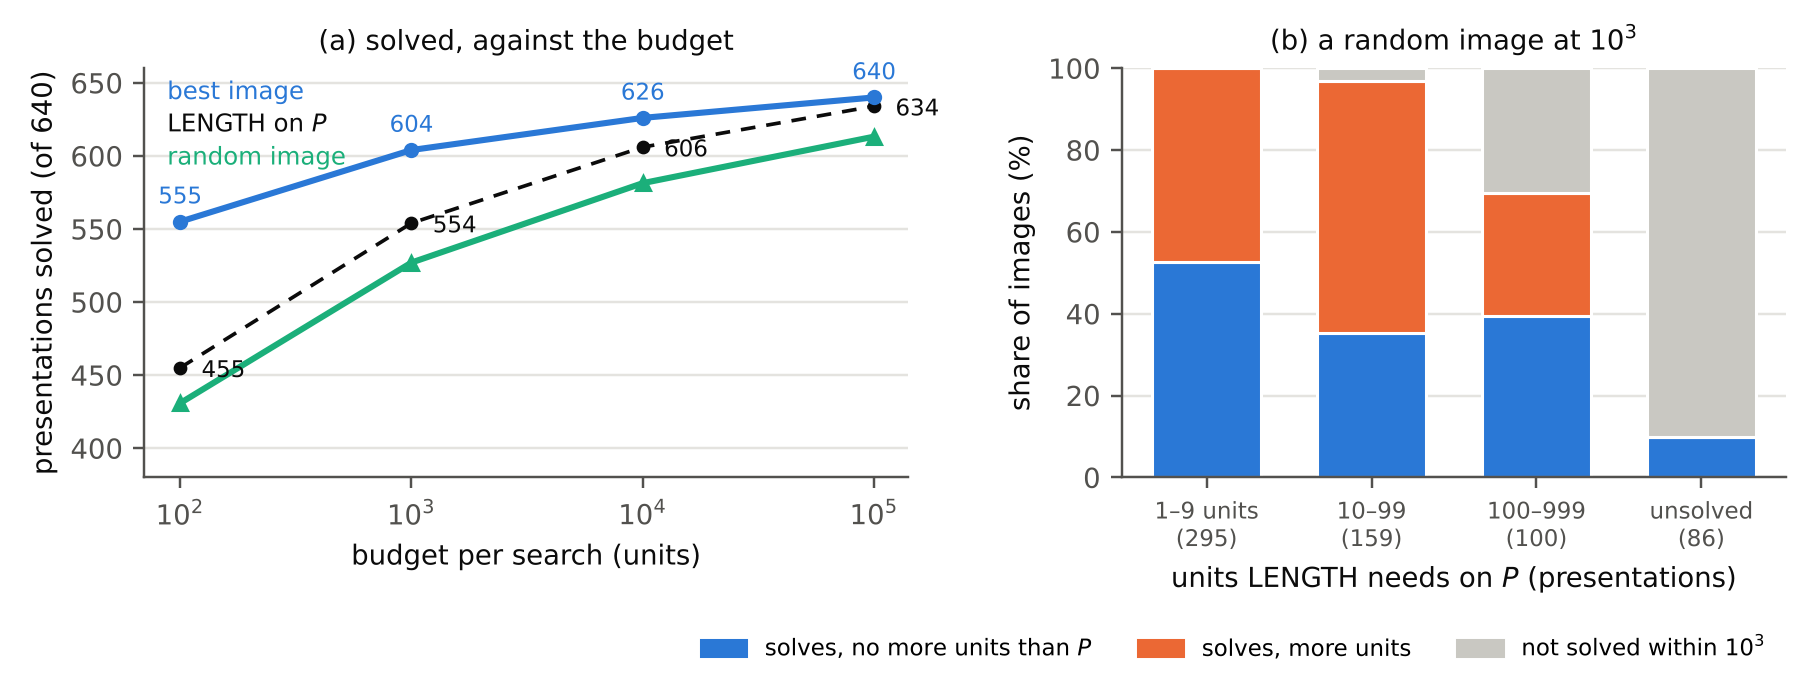
\includegraphics[width=\textwidth]{figures/cov_images.png}
\caption{Every image on MS640. (a) Presentations solved by LENGTH on $P$, by the best image, and by a random image
($640$ times the mean share of a presentation's images solved). (b) A random image against LENGTH on $P$ at budget
$10^3$, with MS640 grouped by the units LENGTH needs on $P$; compare Figure~\ref{fig:stable_split}.}
\label{fig:cov_images}
\end{figure}

The best image passes LENGTH at every budget, but the margin falls from $100$ to $6$, and finding the image costs more
than the margin (Table~\ref{tab:cov_all}, Figure~\ref{fig:cov_images}a). Unlike a stable start, an image is often
cheaper than $P$ (Figure~\ref{fig:cov_images}b): where LENGTH needs $1$ to $9$ units, $52.6\%$ of the images solve in
no more units, and where LENGTH fails within $10^3$, $9.8\%$ of the images still solve.

\paragraph{The best image, then LENGTH.} Search each presentation from its best image only. Then LENGTH solves all
$640$ presentations of MS640 within $14{,}473$ units each, $295{,}268$ units in all (mean $461$, median $7$), with
paths of median $6$ and at most $489$ S-moves. LENGTH on $P$ still misses $6$ at $10^5$ units.
\begin{center}
\small
\begin{tabular}{lrrrrrr}
\toprule
budget (units) & $10$ & $10^2$ & $10^3$ & $10^4$ & $3\cdot10^4$ & $10^5$\\
\midrule
best image, then LENGTH & $416$ & $555$ & $604$ & $626$ & $640$ & $640$\\
LENGTH on $P$ & $317$ & $455$ & $554$ & $606$ & $626$ & $634$\\
\bottomrule
\end{tabular}
\end{center}
The last $36$ presentations are the rows with $n=7$, $r_1=y^{-8}x^{-1}y^{7}x$; their best images need about
$14{,}400$ units and give paths of $489$ S-moves. The best image is chosen with hindsight: finding it by searching every
image costs a mean of $657{,}198$ units per presentation at budget $10^5$.
